\chapter{基于Hyperledger Fabric的区块链云化框架}

本章首先通过快速评审获得Kubernetes operator赋能质量属性的策略集,  随后阐述区块链云化的原则, 最后提出基于Hyperledger Fabric的区块链云化框架。

\section{快速评审}\label{section: rapid_reviews}

软件工程中, 快速评审(Rapid reviews)是一种轻量级的二级研究, 以实践为导向专注于及时的向研究人员提供证据\cite{cartaxo2020rapid}。本文对已发表的学术文章进行快速评审, 快速评审的目的是为了在较短时间内了解目前学术界使用Kubernetes operator进行云化的现状, 以及如何使用Kubernetes对现有系统进行赋能。随后, 对应文献对快速评审所得到的结果进行整理归纳得到Kubernetes operator如何为质量属性赋能的策略集。

本文的快速评审过程分为以下步骤: 首先进行自动化的全文数据库检索, 再筛选出与Kubernetes operator及架构改造强相关的文献, 接下来提取出本文所关注的质量属性及相关策略, 最后归纳整理出策略集。

{\footnotesize
\begin{longtable}[h]{m{60pt} m{210pt} m{40pt}<{\centering}}
    \caption[每个全文数据库的搜索字符串]{每个全文数据库的搜索字符串} \label{search_string} \\
        \toprule  
        \textbf{全文数据库}&\textbf{搜索字符串}&\textbf{文献数}\\
        \hline
        IEEE Xplore &(“kubernetes AND operator”) OR (“k8s AND operator”) OR (“custom resource defination”) & 23 \\

        ACM & “kubernetes operator” OR “k8s operator” & 7 \\

        Springer &((“kubernetes AND operator”) OR (“k8s AND operator”))AND ((“custom resource defination”) OR "CRD") & 0 \\

        ScienceDirect &(“kubernetes AND operator”) OR (“k8s AND operator”) OR (“custom resource defination”) & 0 \\
        \hline
        Scoups\&Google &“kubernetes operator”& 21(去重) \\
        \bottomrule
    \end{longtable}
}

如表\ref{search_string}所示, 为全面获取学术届对基于Kubernetes operator云化的策略, 确定了本次检索的全文数据库以及搜索字符串。本次检索主要针对计算机与软件工程领域的全文数据库\cite{lisboa2010systematic}(包含ACM、IEEE Xplore、Springer、ScienceDirect), 同时检索Scoups以及谷歌学术进行补充。最终, 围绕“kubernetes operator”为检索主题得到的共51篇论文。在文献筛选阶段, 本文根据筛选标准筛选出15篇与Kubernetes operator云化强相关的文献, 入选文献如表\ref{rapid_reviews}所示。文献筛选标准主要有:

\begin{itemize}[itemindent=2em]
    \item 论文的主要目的是利用Kubernetes对原有系统进行云化;

    \item 论文针对于Kubernetes operator方法;

    \item 论文介绍了具体的改造策略及相关的质量属性。
\end{itemize}

{\footnotesize
\begin{longtable}[h]{m{40pt} m{280pt} m{40pt}<{\centering}}
    \caption[快速评审入选文献列表]{快速评审入选文献列表} \label{rapid_reviews} \\
        \toprule  
        \textbf{文献编号}&\textbf{文献标题}&\textbf{文献引用}\\
        \hline
        [P1]&Enhancement of observability using Kubernetes operator&\cite{Shenoy2022496}\\
        
        [P2]&Designing a Kubernetes Operator for Machine Learning Applications&\cite{kanso2021designing}\\
        
        [P3]&Container orchestration on HPC systems through Kubernetes&\cite{zhou2021container}\\
        
        [P4]&Validation and Benchmarking of CNFs in OSM for pure Cloud Native applications in 5G and beyond&\cite{pino2021validation}\\
        
        [P5]&On-the-fly fusion of remotely-sensed big data using an elastic computing paradigm with a containerized spark engine on kubernetes&\cite{huang2021fly}\\
        
        [P6]&A Role-Based Orchestration Approach for Cloud Applications&\cite{yue2021role}\\
        
        [P7]&A Design of MANO System for Cloud Native Infrastructure&\cite{lee2021design}\\
        
        [P8]&Dynamic Updates of Virtual PLCs Deployed as Kubernetes Microservices&\cite{koziolek2021dynamic}\\

        [P9]&Suture: Stitching safety onto kubernetes operators&\cite{mahajan2020suture}\\
        
        [P10]&Automation of virtualized 5G infrastructure using mosaic 5G operator over kubernetes supporting network slicing&\cite{wiranata2020automation}\\
        
        [P11]&5G Cloud-Native: Network Management \& Automation&\cite{arouk20205g}\\
        
        [P12]&Proposed model for distributed storage automation system using kubernetes operators&\cite{sharma2020proposed}\\
      
        [P13]&Monitoring Resilience in a Rook-managed Containerized Cloud Storage System&\cite{baumann2019monitoring}\\
        
        [P14]&Reproducible Benchmarking of Cloud-Native Applications With the Kubernetes Operator Pattern&\cite{henning2021reproducible}\\
        
        [P15]&Pivotal Greenplum©for Kubernetes: Demonstration of Managing Greenplum Database on Kubernetes&\cite{patel2019pivotal}\\
        \bottomrule
    \end{longtable}
}

在数据提取阶段, 本文对5个提取项(文献标题、文献发表年份、质量属性、策略、所属领域)进行抽取, 共得到44条针对不同质量属性的相关策略。在数据归纳阶段, 由于不同的文献中对语义相同的质量属性用词存在明显差异, 本文根据国际软件质量评价标准ISO/IEC 25010:2011\footnotemark[1]\footnotetext[1]{\href{https://www.iso.org/standard/35733.html}{ISO/IEC 25010:2011 System and software quality models}}所定义的质量模型对收集到的文献中表述的质量属性进行映射, 同时对相同或相似的策略进行整理合并, 得到策略集如表所示。

{\footnotesize
\begin{longtable}[h]{m{40pt}|m{40pt}|m{20pt}|m{150pt}|m{80pt}}
    \caption[策略集]{策略集} \label{policy_set} \\  
        \hline
        \textbf{文献中质量属性}&\textbf{ISO质量属性}&\textbf{编号}&\textbf{策略}&\textbf{参考文献}\\
        \hline
        \multirow{4}*{\parbox[c]{40pt}{生产效率 \\ 效率}} & \multirow{4}*{易部署性}
        &S1&容器化 & [P3] \\\cline{3-5}
        & &S2&自动化配置复杂领域知识 & [P1, P2, P12-15] \\\cline{3-5}
        & &S3&自动化构建、部署应用程序 & [P6, P10, P11] \\\cline{3-5}
        & &S4&operator与helm结合 & [P1, P4, P13] \\\cline{3-5}

        \hline
        可迁移性 & 适应性
        &S5&容器化及Kubernetes特性 & [P1-P3, P8, P10-P12] \\\cline{3-5}

        \hline
        \multirow{3}*{\parbox[c]{40pt}{可伸缩性 \\ 灵活性}} & \multirow{3}*{无}
        &S6&容器化及Kubernetes特性 & [P2-P5, P7, P12] \\\cline{3-5}
        & &S7&基于监控指标并进行伸缩处理 & [P2, P6, P13] \\\cline{3-5}
        & &S8&基于PVC及StorageClass的存储扩容 & [P15] \\\cline{3-5}

        \hline
        \multirow{4}*{安全性} & \multirow{4}*{安全性}
        &S9&RBAC & [P2] \\\cline{3-5}
        & &S10&自定义访问控制机制 & [P9] \\\cline{3-5}
        & &S11&多用户认证授权机制 & [P3, P13] \\\cline{3-5}
        & &S12&资源隔离 & [P13] \\\cline{3-5}

        \hline
        \multirow{2}*{可用性} & \multirow{2}*{可靠性}
        &S13&基于Kubernetes自愈能力 & [P2, P15] \\\cline{3-5}
        & &S14&主备切换 & [P15] \\\cline{3-5}

        \hline
        \multirow{1}*{可监控性} & \multirow{1}*{无}
        &S15&基于Prometheus的监控体系 & [P1, P5, P12] \\\cline{3-5}
        \hline
    \end{longtable} 
}


访问控制是提供云数据安全和隐私的一种基本方法, 可以防止未经授权的用户侵入云数据。不可靠的访问控制方法也会影响其他功能, 如身份验证、授权和数据审核。云中的传统访问控制方法主要基于成熟的访问控制策略, 现有的传统访问控制策略分为四个方面: 

自主访问控制(DAC)、强制访问控制(MAC)、基于角色的访问控制(RBAC)和基于属性的访问控制(ABAC)。在DAC中,合法用户(如服务提供商)负责确定其他用户如何访问对象(如云用户)[79]。通过这种方法,由于DAC不需要严格的规则,实现了对云用户的灵活访问控制。与DAC相反,MAC是通过预定义的信任策略实现的,该策略不能动态更改。系统管理员负责访问控制而不是对象,因此该方法关注的是自信而不是完整性[24]。

对比表, 资源隔离


\section{设计原则}\label{section: framework_characteristics}

区块链云化框架致力于在BaaS一站式构建、管理、托管和运维区块链网络及其应用的基础上更深入云原生底层基础设施Kubernetes的底层, 有效利用云能力对Fabric基础设施赋能, 需要满足以下原则:

\begin{itemize}[itemindent=2em]
    \item 易用性: 在Kubernetes上启动管理Hyperledger Fabric网络并部署链码需要专业的领域知识, Fabric各组件的配置项繁多且与Kubernetes适配极易出错。区块链云化框架需屏蔽底层Fabric配置与Kubernetes逻辑, 帮助用户采用命令行配置的方式提供完整的Fabric各组件的全生命周期管理;

    \item 可迁移性: 区块链云化框架需要具备基础架构的云独立性, 本框架依托Kubernetes, 可以方便的迁移到支持Kubernetes的任何云;

    \item 可视运维: 当前区块链系统缺乏一套涵盖不同层面的标准方法来监控区块链及其智能合约的运行\cite{zhangfuli2021smartcontract}。 区块链云化框架需提供基本运维能力, 有效复用云上监控方案为区块链系统提供7*24小时可视化资源监控能力;

    \item 安全性: 区块链云化框架需要具备有效的认证、鉴权、准入机制来确保区块链系统的安全性; 具备可插拔的共识算法取保区块链的去中心化、可追溯等特点, 支持完善的用户密钥授权、保存、隔离处理以及提供可靠的故障恢复能力;

    \item 可扩展性: 区块链云化框架需按照模块化配置, 将Kubernetes底层的计算资源、存储资源、网络资源等供给Fabric, Fabric的Ca、Peer、Orderer基本组件的证书认证、共识、TLS加密、存储等功能模块作为可配置项进行命令式配置; 该框架能够确保系统核心底层逻辑稳定运行的同时, 对外提供小而精的扩展边界, 实现系统的高内聚与低耦合;

    \item 透明性: 区块链云化框架需保证区块链上所有的交易记录是可追溯的、不可篡改的, 区块链交易过程以及获取交易产生的记录需要专业人员才能获取操作, 非专业人员难以理解, 框架需通过简单透明的方式获取交易记录。
\end{itemize}

\section{基于Hyperledger Fabric的区块链云化框架}

\begin{figure}[h] %figure环境,h默认参数是可以浮动,不是固定在当前位置。如果要不浮动,你就可以使用大写float宏包的H参数,固定图片在当前位置,禁止浮动。
    \centering %使图片居中显示
    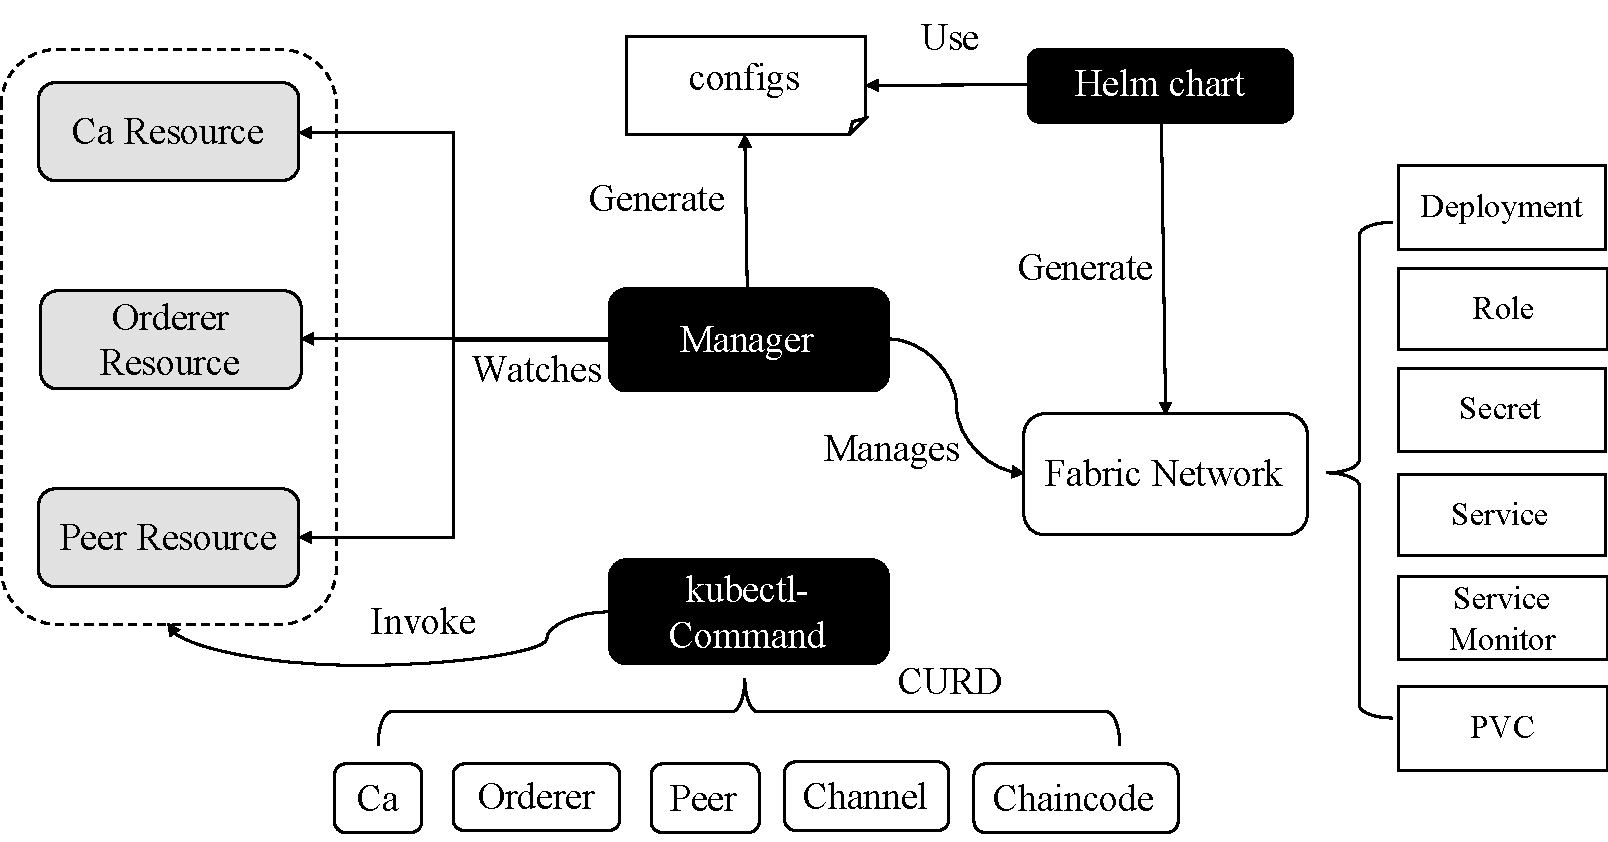
\includegraphics[width=1.0\textwidth]{FIGs/chapter3/framework.pdf} %中括号中的参数是设置图片充满文档的大小,你也可以使用小数来缩小图片的尺寸。
    \caption{基于Hyperledger Fabric的区块链云化框架} %caption是用来给图片加上图题的
    \label{framework} %这是添加标签,方便在文章中引用图片。
\end{figure}%figure环境

结合\ref{section: rapid_reviews}所调研的策略集并基于\ref{section: framework_characteristics}所述原则, 如图\ref{framework}所示, 本文提出了基于Hyperledger Fabric的区块链云化框架。利用k8s operator方法将领域知识集成到Kubernetes API编排过程中\cite{henning2021reproducible}。k8s API是云原生容器管理系统的大脑, 它是一个复杂的API, 具有多个层与各种资源\cite{Yilmaz2021}。该框架重点整合\ref{section: BaaS}节所展示的BaaS区块链层Fabric的联盟链能力以及计算资源层k8s的计算资源、存储资源等资源为上层的区块链服务层提供完备的去中心化应用开发的能力。同时该框架能够隐式管理密码文件、按需配置调度k8s资源, 解决Fabric部署效率、安全性、弹性等运营难题, 节约开发人员以及运维人员时间成本, 使得其更加专注于去中心化应用的逻辑。

Operator应该管理单一类型的应用程序, 遵循UNIX原则:只做一件事, 并把它做好\cite{d2020design}。本框架必须解决的主要任务是屏蔽Fabric及k8s底层细节, 简化Fabric网络的各节点的部署, 以及有效利用k8s代码化及云化的管理基础设施, 所以本框架需要分别对Ca、Orderer、Peer三种不同的网络组建分别进行完整生命周期管理。

本框架的整体工作流程将分为几个步骤。首先, 根据S2将Fabric领域知识注入CRD, 这些属性包含Fabric网络中Ca、Orderer、Peer各节点所具备的功能、性能、监控等各方面。将CRD作为本框架的输入, 通过自定义kubectl命令完成静态CRD相关属性的配置。其次, Manager是本框架的处理单元, 其被设计成一个黑盒\cite{yu2020system}, 用户无需关心Manager的内部逻辑设计。结合S3及S4, Manager自动生成部署配置文件, 使用生成的配置文件并结合Helm chart可以轻松的将Fabric网络各节点部署进目标k8s集群。除了部署之外, 利用S15所述策略,   Manager将持续监控这些节点及其存储资源。根据持续监测结果并调用k8s及Fabric API将各节点调整到期望状态以维持Fabric网络的稳定。最后, Fabric网络是本框架的输出, 通过自定义kubectl命令完成动态通道、链码的增删查改。除Fabric网络各节点基本Deployment、Service外, 本框架采用istio专用基础设施层完成高性能、适应性和可用性\cite{li2019service}\cite{larsson2020impact}的TLS通信负载均衡; 采用原生Role、Secret、PVC的方式管理Fabric网络的权限、密码及存储。

\subsection{Custom Resource Definition}\label{section: Custom_Resource_Definition}

CRD通过扩展k8s API将具备领域知识资源类型注入进k8s集群中。k8s提供了标准资源ConfigMap, 也可用于使配置数据项供应用程序使用, 但这两种针对不同的情况。ConfigMap擅长为在集群上的pod中运行的程序提供配置, 应用程序通常希望从pod中读取此类配置, 例如文件或环境变量的值, 而不是从Kubernetes API中读取。CRs由标准的k8s客户端创建和访问, 遵守k8s规范。通过自定义controller可以监控CRs运行, 这些代码可以反过来创建、更新或删除其他集群对象, 甚至集群外的任意资源。

本框架基于Fabric网络各节点自身功能及配置\footnotemark[1]\footnotetext[1]{\href{https://github.com/hyperledger/fabric-ca/blob/main/cmd/fabric-ca-server/config.go}{Ca Config}}\footnotemark[2]\footnotetext[2]{\href{https://github.com/hyperledger/fabric/blob/main/sampleconfig/orderer.yaml}{Orderer Config}}\footnotemark[3]\footnotetext[3]{\href{https://github.com/hyperledger/fabric/blob/main/sampleconfig/core.yaml}{Peer Config}}设计三种Fabric静态资源类型作为输入, 篇幅原因仅展示包括但不限于如表\ref{crd_description}所示的属性。额外的, 除上述针对不同网络节点的特殊属性外, 本框架需要为每个节点提供如副本数、镜像、Hosts、日志、ServiceMonitor等基本属性维持上述网络节点的基本运行状态。

{\footnotesize
\begin{longtable}[h]{m{60pt}|m{100pt}|m{210pt}}
    \caption[CRD描述]{CRD描述} \label{crd_description} \\
        \hline   
        \textbf{CRD名称}&\textbf{属性}&\textbf{描述}\\
        \hline
        \multirow{8}*{Ca Resource}
        & CRLSizeLimit & 可接受证书撤销列表(Certificate Revocation List, 简称CRL)的大小限制 \\\cline{2-3}
        & TLS & 服务器侦听TLS端口以及证书等信息 \\\cline{2-3}
        & CA & 包含与证书颁发机构相关的信息 \\\cline{2-3}
        & Database & 用作数据存储 \\\cline{2-3}
        & CFG & 配置身份允许的错误密码尝试次数 \\\cline{2-3}
        & CSR & 控制根CA证书的创建, 如根CA证书的过期时间配置 \\\cline{2-3}
        & Registry & 部分控制fabric-ca服务器执行验证包含用户名和密码的注册和检索标识的属性名称、值的方式 \\\cline{2-3}
        & BCCSP & 用于选择要使用的加密库实现 \\\cline{2-3}
        \hline  
        \multirow{4}*{Orderer Resource} & Genesis & 初始区块相关配置 \\\cline{2-3}
        & BootstrapMethod & 指定了获取引导块系统通道的方法 \\\cline{2-3}
        & ChannelParticipation & 通道管理对系统链码的依赖 \\\cline{2-3}
        & Secret & 包含Orderer的数字签名以及与Ca通信所需的基本信息\\\cline{2-3}
        \hline 
        \multirow{6}*{Peer Resource} & Gossip & 确保Peer间通过Gossip协议来达到所有账本的最终一致性 \\\cline{2-3}
        & LevelDB/CouchDB & Fabric提供levelDB与CouchDB用以保存Fabric账本信息, 用以灵活适应Peer不同数据库之间的转换 \\\cline{2-3}
        & CouchDBExporter & 采集CouchDB的监控数据 \\\cline{2-3}
        & ExternalChaincodeBuilder & 提供外部链码构建的能力 \\\cline{2-3}
        & Secret & 包含Peer的数字签名以及与Ca通信所需的基本信息\\\cline{2-3}
        \hline 
    \end{longtable} 
}

\subsection{Manager}

CRs本身仅为特定应用程序提供声明式API的数据项的集合, controller负责对CRs的不同事件做出反馈, 管理CRs的完整生命周期。

\begin{figure}[h] %figure环境,h默认参数是可以浮动,不是固定在当前位置。如果要不浮动,你就可以使用大写float宏包的H参数,固定图片在当前位置,禁止浮动。
    \centering %使图片居中显示
    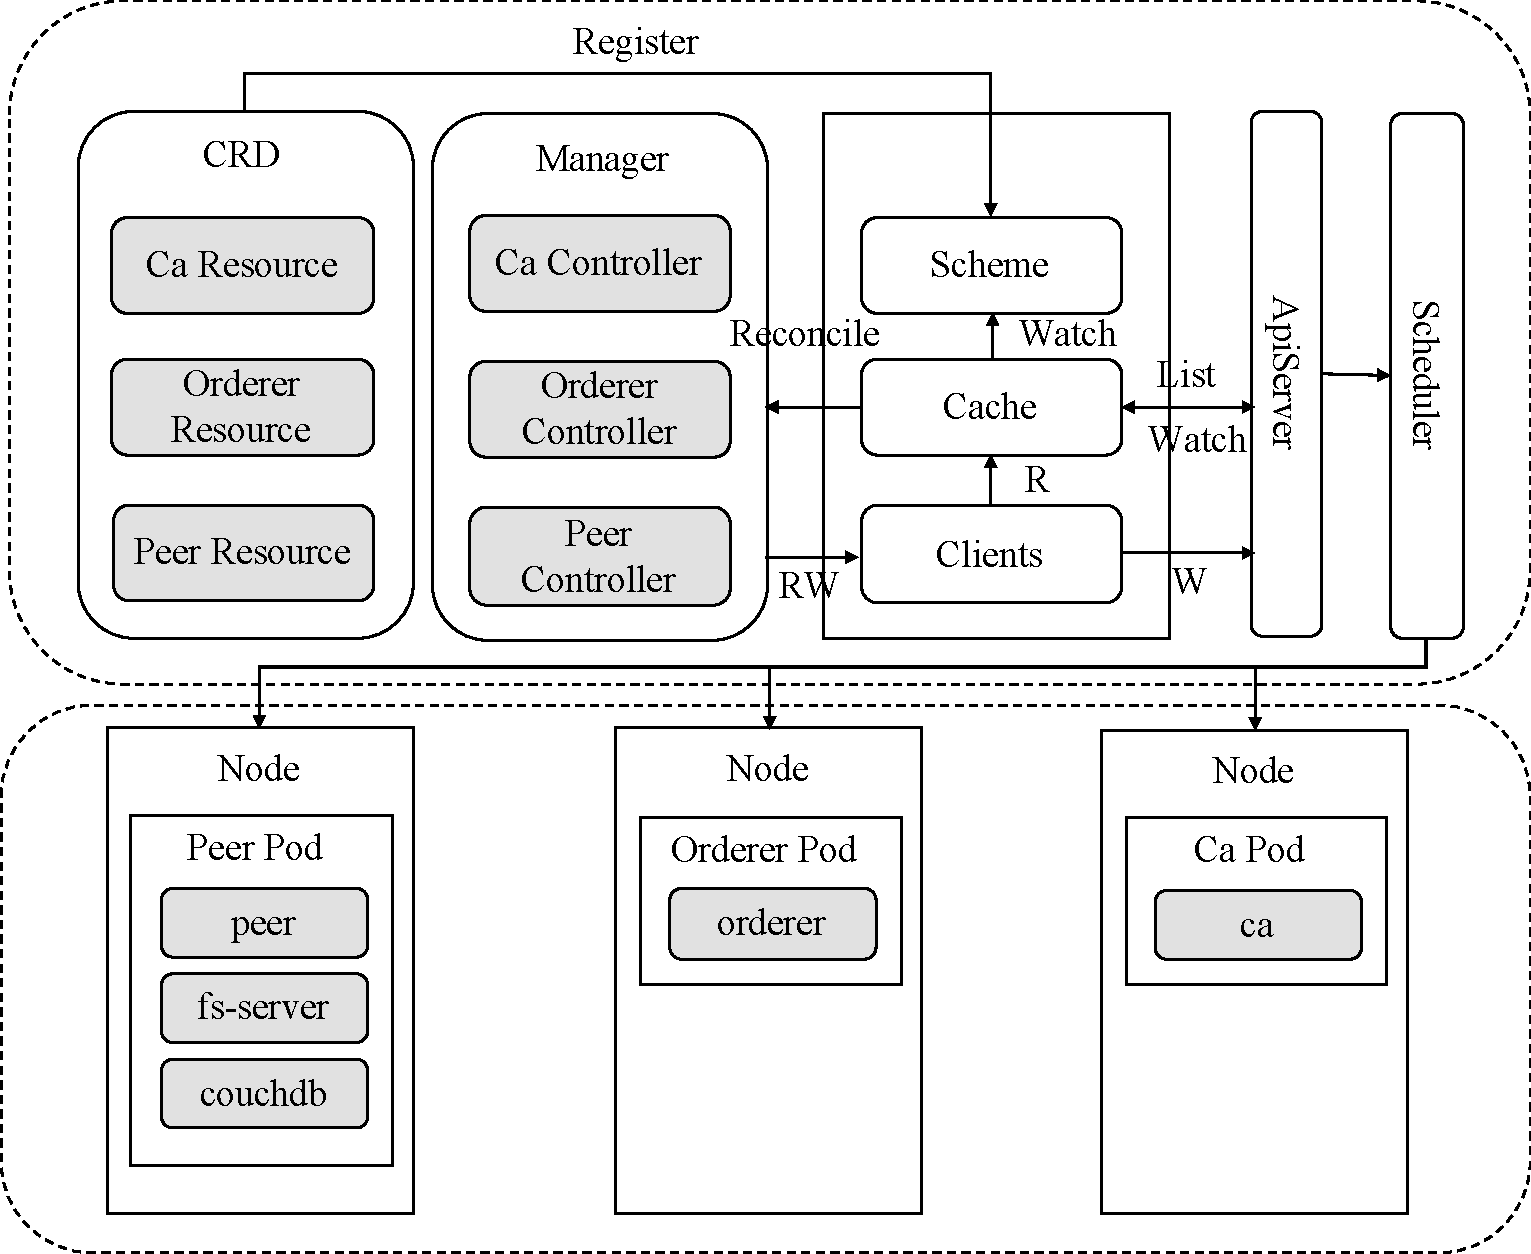
\includegraphics[width=0.95\textwidth]{FIGs/chapter3/manager.pdf} %中括号中的参数是设置图片充满文档的大小,你也可以使用小数来缩小图片的尺寸。
    \caption{Manager监听CRs} %caption是用来给图片加上图题的
    \label{manager} %这是添加标签,方便在文章中引用图片。
\end{figure}%figure环境

如图\ref{manager}所展示的是Manager监听CRs的全过程。首先, 需要在CRs中指定Fabric网络各节点所期望的状态, CRD会注册进入Scheme, 其提供了ApiServer对应的集群中GVK(Group Version Kind, k8s集群资源定义方式)与CRs资源类型的映射, 通过资源类型controllers就能获取CRs所定义的期望状态; 其次, cache通过List-Watch机制与ApiServer进行通信用以同步监听Fabric网络各节点在k8s集群中的创建、删除、更新等操作, cache可以获取Fabric网络各节点的实际状态; 最后, controller循环监听期望状态与实际状态, 若期望状态与实际状态不一致, 则通过调用clients更新、缩放、扩展、备份等操作进行协调一致。

为提升区块链云化框架的生产效率, 本文根据S3、S4设计了一套针对Fabric网络各节点helm的通用CRD与controller, 直接将提前配置好的helm随CRD以及controller一直部署进k8s。Helm通过调用k8s的ApiServer逐个将helm chart中的yaml推送给k8s, 当且仅能进行安装。所以helm的弊端是缺乏对资源的全生命期监控, 只有CRD才能持续的监听k8s资源对象的变化事件, 进行全生命期的监控响应, 高可靠的完成部署交付。一旦创建新的CR, controller根据对应的资源对象更新helm的模板参数并重新部署入k8s集群。图\ref{controller}以spec.size为例展示了controller更新helm的流程。本框架不仅通过helm简化部署流程, 并且还能实现带全生命周期管理的helm效果。

\begin{figure}[h] %figure环境,h默认参数是可以浮动,不是固定在当前位置。如果要不浮动,你就可以使用大写float宏包的H参数,固定图片在当前位置,禁止浮动。
    \centering %使图片居中显示
    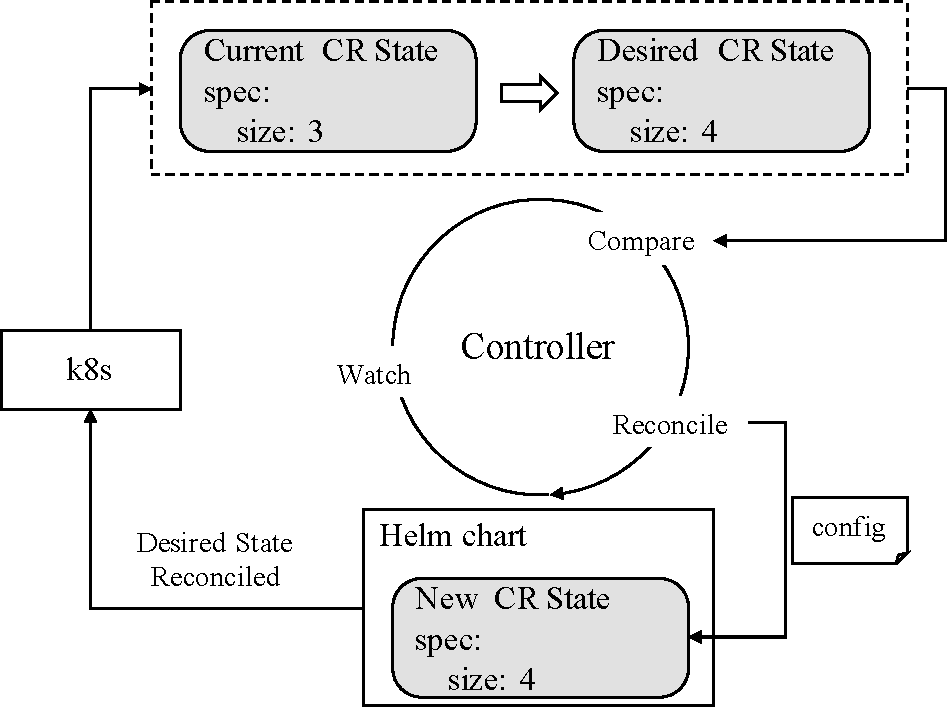
\includegraphics[width=0.75\textwidth]{FIGs/chapter3/controller.pdf} %中括号中的参数是设置图片充满文档的大小,你也可以使用小数来缩小图片的尺寸。
    \caption{controller循环监听} %caption是用来给图片加上图题的
    \label{controller} %这是添加标签,方便在文章中引用图片。
\end{figure}%figure环境

% 可迁移性
在可迁移性方面, 容器化在云原生应用程序中的拥有更高的部署效率\cite{zhou2021container}以及更高的可迁移性, 容器化将应用程序及其库、配置文件和其他依赖项封装在一起, 确保了环境兼容性, 从而使用户能够轻松地在集群之间移动和部署程序。根据S5所示策略, 区块链云化框架遵循标准化原则, 复用Fabric网络各节点镜像并利用k8s进行编排和管理底层的物理资源。这可以确保区块链系统基础架构的云独立性, 取消BaaS平台对云提供商的强依赖性, 提升本框架的的灵活性与通用性。

% 安全性


% 在RBAC模型中,访问权限是根据受试者在系统中的角色和责任分配给他们的,而不是他们的身份[24]。RBAC的本质导致了这一缺陷,因为它缺乏对主体其他方面的考虑。ABAC被提议进一步解决这些问题。它根据对象和主题的属性分析配置访问规则[80]。ABAC的主要优点与认证过程中的综合考虑有关。尽管ABAC的认证是一个耗时的过程,但在云环境中,它花费的计算资源可以忽略不计。

% 智能合约的部署采用的是纯手工或脚本部署的方式, 交易方对生产部署环境有不同的要求,缺乏提高部署效率、缩短产品交付周期的有效工具与方法。同时, 区块链领域频繁的出现安全问题可能会动摇人们对去中心化应用的信任。虽然智能合约安全事件占比并不高, 但是每次发生安全事件造成的损失能达到数百万乃至上亿美元。最著名的有发生在2016年6月的The DAO\cite{zhao2017dao}安全漏洞, 造成了1.5亿美元的损失,也造成了以太坊的永久性硬分叉。

在安全性方面区块链云化框架复用k8s的原生安全保障体系, 主要涉及到两方面。 一方面是框架对k8s集群操作的访问控制限制, 区块链云化框架会生成很多清单文件向k8s集群中部署Fabric网络, 同时k8s集群需要向已部署的区块链云化框架授予在Fabric网络中生命周期内执行各种任务的权限。k8s没有以用户身份进行身份验证, 如图\ref{safety}-I所示, 本框架采用基于角色的权限控制(Role-Based Access Control, 简称RBAC)将对k8s资源操作的最小权限映射到框架中的Manager及Fabric网络节点, 在允许框架正常工作的同时, 应尽可能限制访问; 另一方面是Fabric网络运行环境均受k8s安全容器保护。在密码管理方面, 框架避免使用直接向节点镜像中注入环境变量的方式管理密码信息。如图\ref{safety}-II所示, 以注册Fabric网络用户为例, 本框架采用Secret配合x509\cite{8249485}存储管理敏感数据, 这种方式不但能提高灵活性而且增加了密码的传输、存储、访问安全, 增强隐私保护。

\begin{figure}[h] %figure环境,h默认参数是可以浮动,不是固定在当前位置。如果要不浮动,你就可以使用大写float宏包的H参数,固定图片在当前位置,禁止浮动。
    \centering %使图片居中显示
    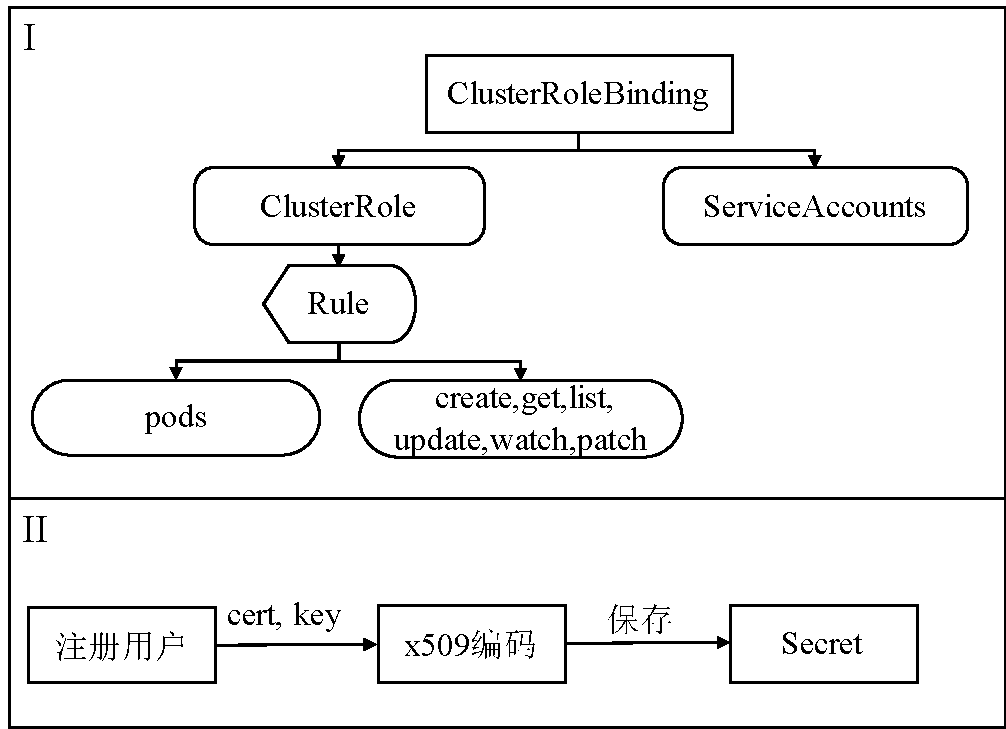
\includegraphics[width=0.75\textwidth]{FIGs/chapter3/safety.pdf} %中括号中的参数是设置图片充满文档的大小,你也可以使用小数来缩小图片的尺寸。
    \caption{区块链云化框架的安全性} %caption是用来给图片加上图题的
    \label{safety} %这是添加标签,方便在文章中引用图片。
\end{figure}%figure环境

% 扩展性设计
% 从海量数据存储的角度来看,使用云存储是加强区块链系统的一种替代方法,它减少了因区块存储空间有限而造成的限制。关键问题是确定哪些数据应存储在块中,以便在块大小和区块链功能之间取得巨大平衡。
% 在本节中,我们讨论了解决区块链存储限制的链外解决方案。应用链外存储有利于区块链的可扩展性、存储效率和验证速度。正如我们在之前的文献中所看到的,在设计链上/链下系统时,数据安全和区块链系统效率之间的权衡是一个基本问题。存储多种类型的相关元数据可以确保链外数据的安全性和可控制性。然而,链上的大量数据可能会降低区块链的可伸缩性和效率。因此,如何在链上选择合适的数据来解决安全性和可伸缩性问题可能是未来的研究方向
% Storage as a Service

除\ref{section: Custom_Resource_Definition}所提到的利用CRD对Fabric网络配置进行模块化设计外, 本框架为每个运行中的Fabric网络节点选择配置的PVC, 并为每个PVC中预留出一定的额外存储资源。相较于对所有持久存储的服务使用一个PVC而言, 虽然分配存储远超必要范围增加额外的存储资源冗余, 但用拥有更对的PVC能够保障每个网络节点拥有足够的存储空间, 以便在不缺乏存储资源的情况下正确运行节点。拥有更多的PVC增加了首次部署难度及过度调配的风险, 但多PVC能够灵活针对不同节点运行情况利用k8s进行有针对性的存储扩容, 增强框架对于存储的扩展性。尽管多PVC在管理方面存在一定的复杂性, 但在选择多PVC更加符合最佳实践, 并且效率更高\cite{d2020design}。

% 可视化运维
Prometheus\cite{sukhija2019towards}作为云原生领域的监控事实标准, 有着强大的功能和良好的生态。
Grafana可以与各种其他类似于Prometheus的数据源进行交互并进行可视化。本框架采用非介入式的云上监控方案Prometheus以及Grafana进行可视运维, 在CRD中预留exporter、ServiceMonitor等属性, 对应的在helm chart中定制抓取周期的相关配置对Fabric网络中的Ca、Orderer、Peer、CouchDB等进行可视化监控。同时, Grafana开源特性能够创建自定义插件, 一定程度上能提升本框架的可视运维的灵活度。


\subsection{Fabric网络}

Fabric网络一个复杂的分布式系统, 需要权衡速度、性能等条件对不同网络节点的部署状态进行合理设计。静态节点Ca、Orderer、Peer在首次启动网络时就需要部署在k8s集群中并以Pod形式运行。Pod是k8s中可以创建和部署的最小单位。在k8s集群中, Pod有两种运行状态:

\begin{itemize}[itemindent=2em]
    \item Pod中运行单容器: 每个Pod一个容器是最常见的状态, 在这种状态下, 可以将Pod当作单容器进行封装, 但k8s管理仍然是Pod而不是容器;

    \item Pod中运行个容器: 当容器间需要紧密协作时可以在同一Pod中运行多容器。
\end{itemize}

Ca是Fabric的证书授权中心, Orderer负责交易的排序, 这两个节点在配置上需要满足可插拔式设计。 但在网络运行时, 需要各自在一个Pod中运行即可, 同时 在一个Pod中运行可以有效的利用k8s的自动缩放功能进行弹性伸缩。

Peer是Fabric中被使用最多的模块, 是Fabric网络的基石, 其负责区块链数据的存储以及运行链码。由于Peer节点需要频繁的账本存储单元如CouchDB进行交互, 所以peer容器应当与couchdb容器存在于同一Pod中。在同一个Pod中, peer容器与couchdb紧密协作, 拥有相同的存活周期, 更优的, 相同Pod中的不同容器共享进程、IP地址和数据卷, 可以进行频繁的文件和数据交换。Peer支持外部链码部署, 即链码拥有自己独立的Pod运行环境与Peer解耦, 能够纳入智能合约微服务化流程\cite{zhangfuli2021smartcontract}进行快速响应与监控。 

\section{本章小结}

本章首先详细介绍了目前区块链基础设施的现状, 其中包括基础商业化应用工具不完善以及当前云能力对区块链基础设施的赋能乏力。其次, 本章重点介绍了基于Hyperledger Fabric的区块链云化框架所应满足的6条设计原则; 最后, 介绍了云化框架的工作流程、输入单元CRD、处理单元Manager以及输出单元Fabric网络节点运行状态。
本章首先详细介绍了目前区块链基础设施的现状, 其中包括基础商业化应用工具不完善以及当前云能力对区块链基础设施的赋能乏力。其次, 本章重点介绍了基于Hyperledger Fabric的区块链云化框架所应满足的6条设计原则; 最后, 介绍了云化框架的工作流程、输入单元CRD、处理单元Manager以及输出单元Fabric网络各节点运行状态。